\documentclass[12pt,a4paper]{article}
\usepackage[utf8]{inputenc}
\usepackage[english,russian]{babel}
\usepackage{amssymb,amsfonts,amsmath,cite,enumerate,float,indentfirst}
\usepackage{graphicx}
\usepackage{geometry}
\usepackage{systeme}
\usepackage{amsmath}
\usepackage[bottom]{footmisc}
\usepackage{hyperref}
\usepackage{url}

\hypersetup{
	colorlinks,
	citecolor=black,
	filecolor=black,
	linkcolor=black,
	urlcolor=black
}
\geometry{left=2cm}
\geometry{right=1.5cm}
\geometry{top=2cm}
\geometry{bottom=2cm}


\begin{document}
    \begin{titlepage}
		\begin{center}		
			\vfill	
			Санкт-Петербургский политехнический университет \\
			Петра Великого\\
			\vskip 1cm
			Высшая школа прикладной математики и вычислительной физики \\
			Кафедра «Прикладная математика и информатика»
			\vfill
			\textbf{Дополнение\\
				по лабораторной работе №3\\
				по дисциплине\\
				«Интервальный анализ»\\}
			\vfill
		\end{center}
		\vfill
		\hfill
		\begin{minipage}{0.4\textwidth}
			Выполнил студент:\\
			Лапотников Павел Вадимович\\
			группа: 5030102/90201\\
		\end{minipage}
		\vfill
		\hfill 
		\begin{minipage}{0.4\textwidth}
			Проверил:\\
			к.ф.-м.н., доцент\\
			Баженов Александр Николаевич\
		\end{minipage}
		\vfill
		\hfill 
		\begin{center}
			Санкт-Петербург\\2022 г.
		\end{center}
	\end{titlepage}
	
	\tableofcontents
	\listoffigures
	\pagebreak
     
    \section{Постановка задачи}
    
    Дан набор интервальный данных. Считая, что они задают постоянную величину требуется найти оценки данной постоянной величины.

    \section{Теория}
    \subsection{Мода интервальной выборки}
    Мода - значение из выборки, которое встречается наиболее часто. Да подсчета моды используется следующий алгоритм:
    \begin{itemize}
        \item Если пересечение всех интервалов не пусто, тогда это пересечение и есть моды.
        \item Если пересечение всех интервалов пусто, тогда
        \begin{itemize}
            \item Соберем все концы интервалов в один массив Y и отсортируем его 
            \item Построим интервалы $ z_i = [y_i, y_i_+_1]$
            \item Для каждого $z_i$ посчитаем $\mu_i$ - число инетрвалос из исходной выборки, в которой содержится $z_i$
            \item Найдем $\mu = max(\mu_i)$
            \item Объединим все $z_i$, для которых $\mu_i = \mu$
            \item Полученное объединение и есть мода.
        \end{itemize}
    \end{itemize}

    \subsection{Медиана интервальной выборки}

    Интервальная медиана - это интервал со средней (геометрически) накопленной частотой, т.е. сумму накопленных частот слева равна сумме накопленных частот справа:

    \[ \sum_{i=1}^{m-1} \mu_i = \sum_{i=m+1}^{n} \mu_i \]


    где $\mu_i$ - частота интервала  $z_i$ - количество интервалов из заданного вариационного ряда, в которых содержится $z_i$. Если оказалось так что:
    
    \[ \sum_{i=1}^{m} \mu_i = \sum_{i=m+1}^{n} \mu_i \]

    То за медиану берется:

     \[  med(X) = \frac{z_m + z_m_+_1}{2}  \]

     \subsection{Совместность интервальной выборки}
     Для подсчета совместности используется модификация индекса Жаккара для интервальных данных. 

     \[  JK(x) = \frac{wid(\land x_i)}{wid(\lor x_i)}  \]
    
    
    \section{Реализация}
    Лабораторная работа выполнена с помощью встроенных средств языка программирования Python с использованием библиотек matplotlib, intvalpy, numpy, scipy, statsmodels в среде разработки Jupyter Notebook. 


    \section{Результаты}

    \begin{figure}[H]
        \centering
        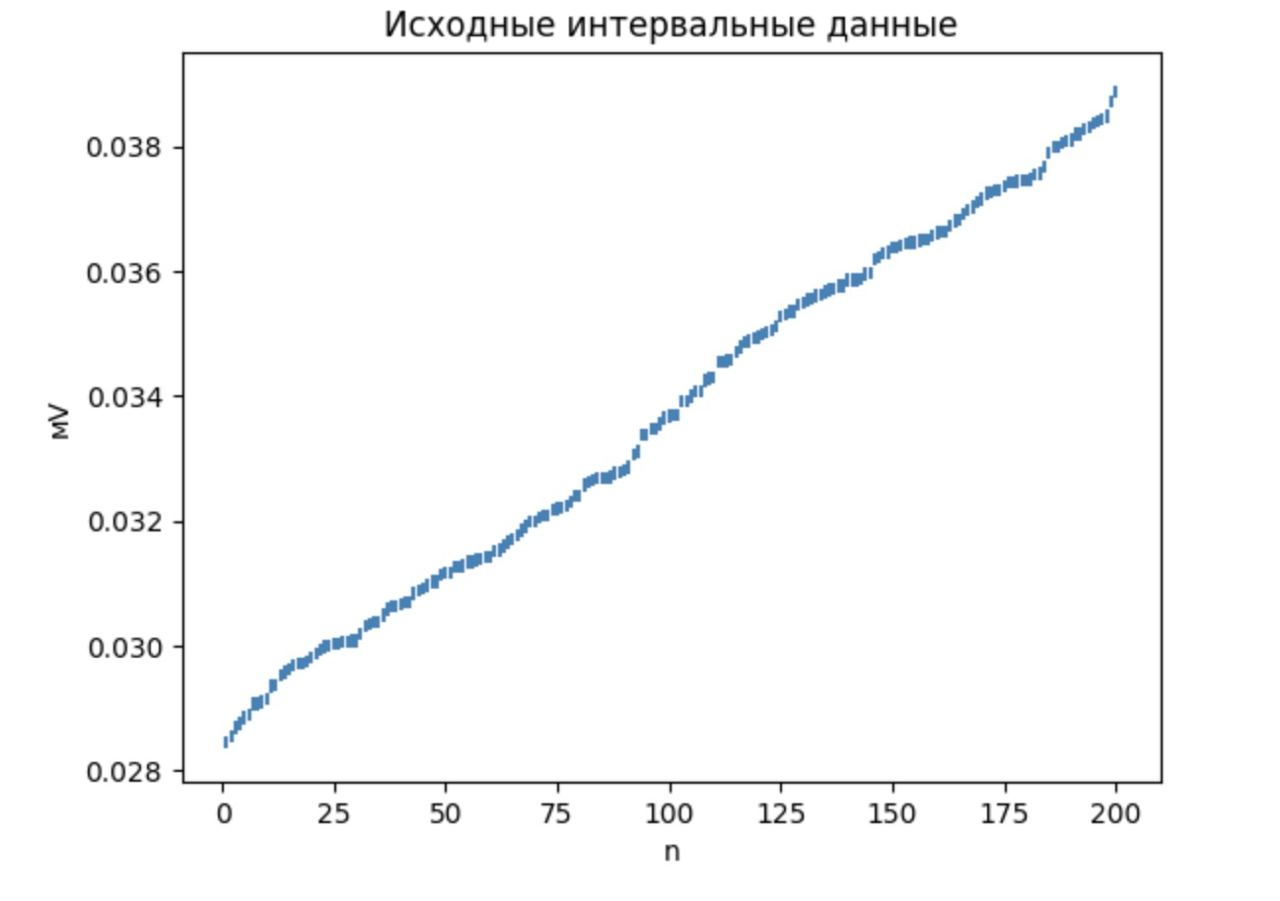
\includegraphics[width=16cm]{3_1.png}
        \caption{График входных интервальных данных}
        \label{fig:box_z}
    \end{figure}

    \begin{figure}[H]
        \centering
        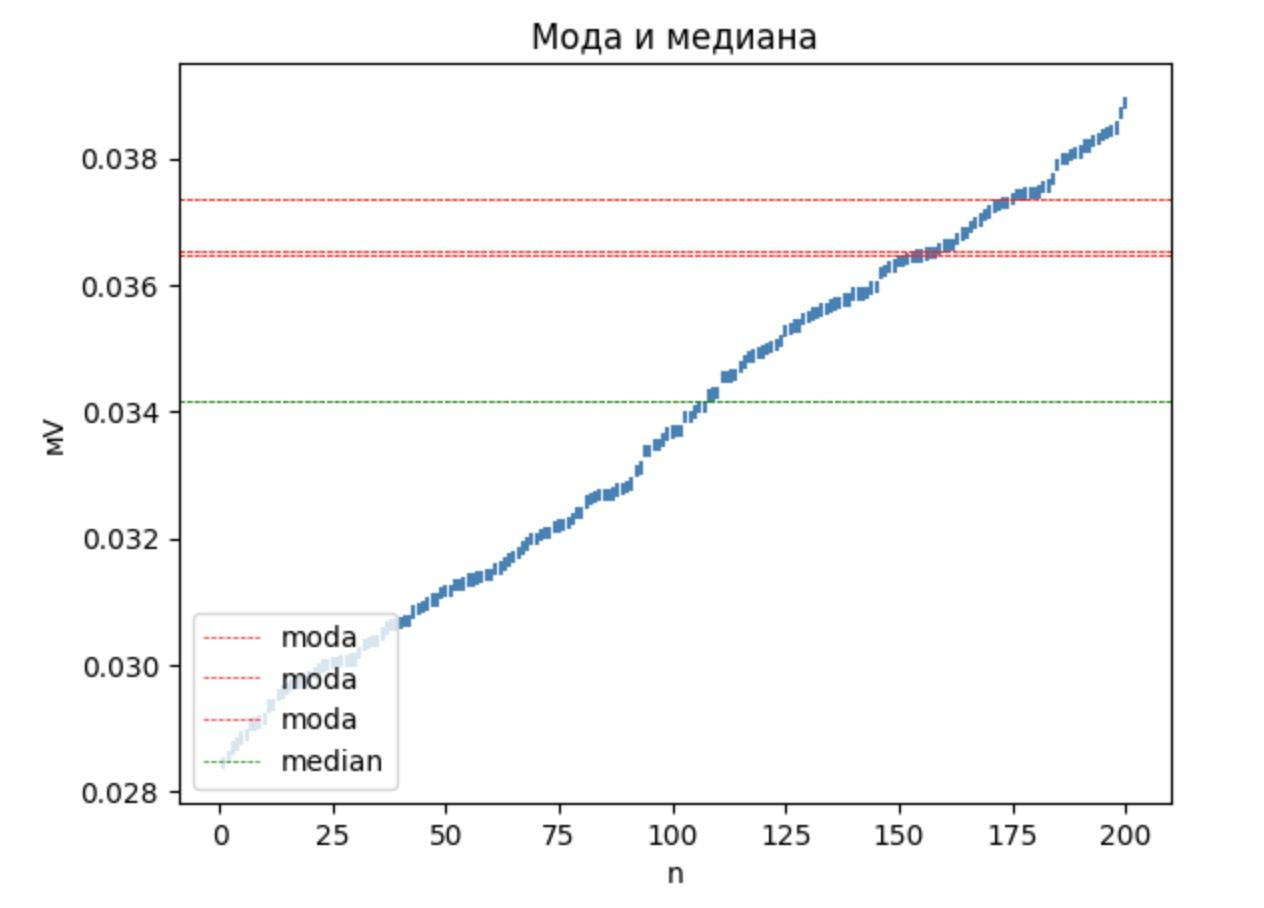
\includegraphics[width=16cm]{3_2.png}
        \caption{График входных интервальных данных с изображенными модой и медианой}
        \label{fig:box_z}
    \end{figure}

    \begin{figure}[H]
        \centering
        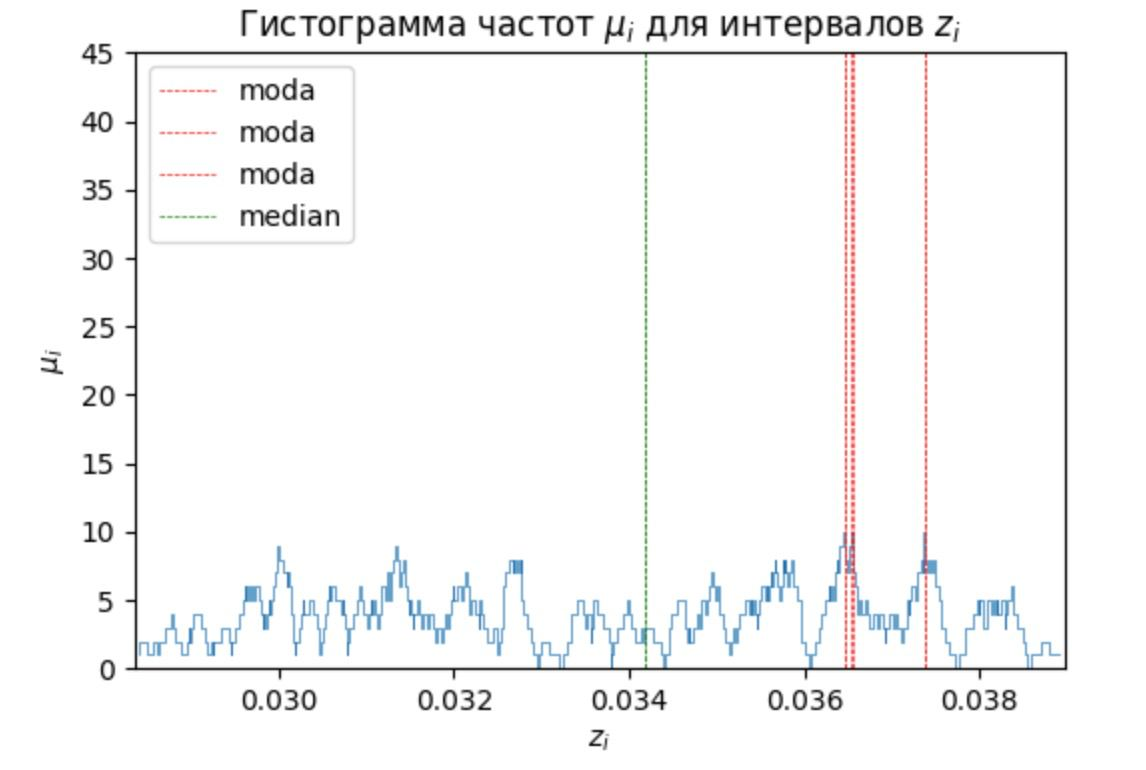
\includegraphics[width=16cm]{3_3.png}
        \caption{Гистограмма частот $\mu_i$ для интервалов $z_i$}
        \label{fig:box_z}
    \end{figure}

    
    
    \subsection{Числовые значения}

    \[  JK(x) = −0.9623139250047104  \]
    \[    med(x) =  [0.0341815, 0.0341845]  \]
    \[    mod(x) = [0.036468, 0.03647] \cup [0.036538, 0.036552] \cup [0.037365, 0.037374]  \]

    \section{Обсуждение}
    \begin{itemize}
        \item По гистограмме частот мы можем сказать что у нас имеется мультимодальное распределение
        \item Сильное различие в положениях медианы и моды также показывает что
выходные данные не задают постоянную величину.
        \item Коэффициент Жаккара близок к 1 - можно сказать что данные не являются совместными, что говорит о том что они не задают постоянную величину.
    \end{itemize}
    \section{Приложение}
        Код программы на GitHub Url https://github.com/lpvmak/interval
\end{document}
